\documentclass[10pt]{article}
\usepackage{../../local}
\urlstyle{same}

\newcommand{\classcode}{Physics C191}
\newcommand{\classname}{Introdcution to Quantum Information}
\renewcommand{\maketitle}{%
\hrule height4pt
\large{Eric Du \hfill \classcode}
\newline
\large{HW 06} \Large{\hfill \classname \hfill} \large{\today}
\hrule height4pt \vskip .7em
\small{Header styling inspired by CS 70: \url{https://www.eecs70.org/}}
\normalsize
}
\linespread{1.1}
\begin{document}
	\maketitle
	\section*{Collaborators}
	I worked with \textbf{David Yang} and \textbf{Teja Nivarthi} on this homeowrk assignment. 
	\section*{Problem 1}
	This problem will have you explore a basic idea in phase estimation algorithms. Imagine that we have a quantum
	computer that implemenets a \( Z \)-rotation of some unknown angle
	\[
		U = \begin{bmatrix} 1& 0\\ 0 & e^{i \theta} \end{bmatrix} 
	\] 
	where \( \theta \) is an unknown phase in the range \( [0, 2\pi] \) that we seek to estimate. We will consider
	 repeatedly applying \( U \) a number \( k \) times, written \( U^{k} \). 
	 \begin{enumerate}[label=\alph*)]
	 	\item What is \( U^{k}\ket*{+} \) written in the computational basis? 

			\begin{solution}
				First, we know that since \( U \) is a diagonal matrix, then:
				\[
					f(U) = \begin{bmatrix} f(u_{11}) & 0 \\ 0 & f(u_{22}) \end{bmatrix} 
				\] 
				So, we can define a function \( f(x) = x^{k} \), which gives us:
				\[
					f(U) = U^{k} = \begin{bmatrix} 1 & 0 \\ 0 & e^{k i \theta} \end{bmatrix} 
				\] 
				Now, applying this to the state \( \ket*{+} \):
				\[
					\frac{1}{\sqrt{2} }\begin{bmatrix} 1 &0\\0&e^{k i \theta} \end{bmatrix} 
					\begin{bmatrix} 1\\1 \end{bmatrix} = \frac{1}{\sqrt{2} }\begin{bmatrix} 
				1\\e^{k i \theta} \end{bmatrix} 
				\] 
			\end{solution}
		\item Identify two projective measurements \( \bra*{m_c} \) and  \( \bra*{m_s} \) such that 
			the output distributions take the forms
			\[
				|\mel{m_c}{U^{k}}{+}|^2 = \frac{1 + \cos(k \theta)}{2}
			\] 
			and 
			\[
				|\mel{m_s}{U^{k}}{+}|^2 = \frac{1 + \sin(k \theta)}{2}
			\] 
			(hint: you may wish to refer back to HW 1 Problem 3). 

			\begin{solution}
				Looking at Homework 1 problem 3, we see that measuring this in the Hadamard basis 
				(that is \( \ket*{+}, \ket*{-}  \)) will give us the desired probabilities. Specifically, we 
				have a state in the form:
				\[
				U^{k}\ket*{+} = \frac{1}{\sqrt{2} }\ket*{0} + \frac{e^{k i \theta}}{\sqrt{2} }\ket*{1}
				\] 
				Transforming this into the Hadamard basis, this state becomes: 
				\begin{align*}
					U^{k}\ket*{+} &= \frac{1}{\sqrt{2} }\left( \frac{1}{\sqrt{2} }(\ket*{+} + \ket*{-}) \right) 
					+ \frac{e^{k i \theta}}{\sqrt{2} }\left( \frac{1}{\sqrt{2} }(\ket*{+} - \ket*{-}) \right) \\
					&= \frac{1 + e^{k i \theta}}{2}\ket*{+} + \frac{1 - e^{k i \theta}}{2}\ket*{-} \\
				\end{align*}
				Then, if we let \( \bra*{m_c} = \bra*{+} \), then the probability of measuremen tis:
				\[
					|\mel{m_c}{U^{k}}{+}|^2 = \left| \frac{1 + e^{k i \theta}}{2} \right|^2 = 
					\cos^2\left( \frac{k \theta}{2}\right) = \frac{1 + \cos(k \theta)}{2}
				\] 
				Then, we can use \( \bra*{-}S \) as the second measurement. This turns out state 
				into:
				\[
					SU^{k}\ket*{+} = \frac{1}{\sqrt{2} }
					\begin{pmatrix} 1 & 0 \\ 0 & i \end{pmatrix} \begin{pmatrix} 1\\e^{k i \theta} \end{pmatrix} 
					= \frac{1}{\sqrt{2} }\begin{pmatrix} 1\\ ie^{k i \theta} \end{pmatrix} 
				\] 
				Now, we convert this into the Hadamard basis: 
				\[
				\ket*{\psi} = \frac{1 + i e^{k i \theta}}{2}\ket*{+} + 
				\frac{1 - i e^{k i \theta}}{2}
				\] 
				So the probability of measuring \( \ket*{-} \) is:
				\[
					|\mel{m_s}{U^{k}}{+}|^2 = \frac{1 + \sin(k \theta)}{2}
				\] 
				as desired. 
			\end{solution}
		\item How can you estimate \( \theta \) for \( k = 1 \)? Why can we not just use a single measurement 
			\( \bra*{m_c} \) or \( \bra*{m_s} \) (hint: think in terms of the unit circle)? 

			\begin{solution}
				For \( k = 1 \), then the measurements are:
				\[
					|\mel{m_c}{U^{k}}{+}|^2 = \frac{1 + \cos(k \theta)}{2} \quad |\mel{m_s}{U^{k}}{-}|^2
					= \frac{1 + \sin (k \theta)}{2}
				\] 
				We can estimate \( \theta \) for \( k = 1 \) by repeatedly creating the state and measuring, eventually 
				we will get the distribution of measuring \( \ket*{+} \) and \( \ket*{-} \), from which we can 
				determine the angle \( \theta \) we're working with. Plotting these two 
				curves together:
				\begin{center}
					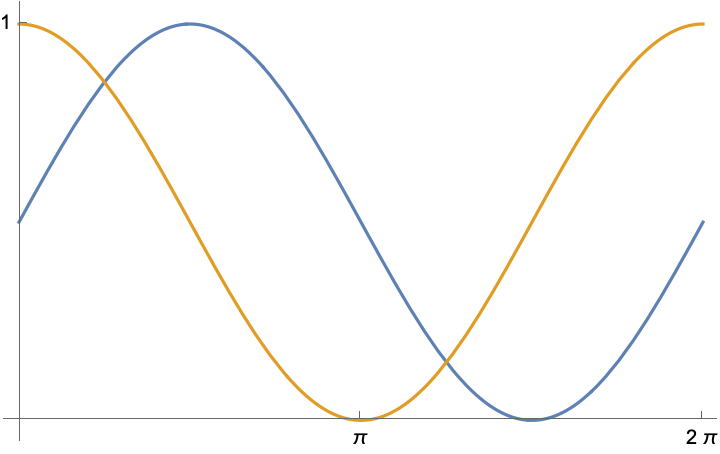
\includegraphics[scale=0.8]{q1c.png}
				\end{center}
				We can see that for any particular value of \( \theta \), the distributions of \( \bra*{m_c} \) 
				and \( \bra*{m_s} \) are distinct, and so with enough repeated measurements we 
				are able to estimate \( \theta \). 
			\end{solution}
		\item What problems arise when trying to estimate \( \theta \) for \( k > 1 \) (hint: it may be 
			useful to draw a picture)?

			\begin{solution}
				For \( k > 1 \), we run into the issue that on the interval \( [0, 2\pi] \), the distribution 
				for \( m_c \) and \( m_s \) look the same for different values of \( \theta \). Here's the plot 
				for \( k = 2 \):
				\begin{center}
					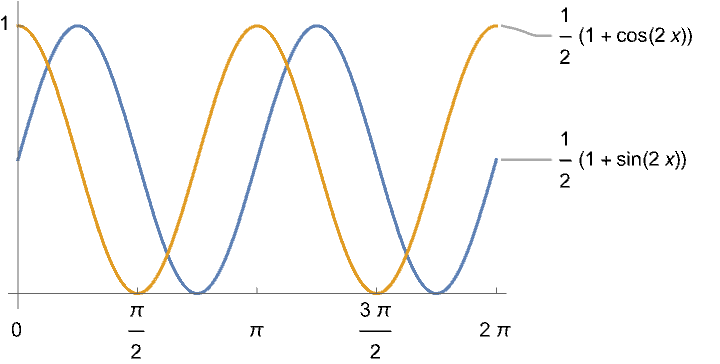
\includegraphics[scale=0.8]{q1d.png}
				\end{center}
				Consider the distribution at \( \theta = \frac{\pi}{2} \). Here, we have that the probability 
				of measuring \( m_c \) is zero and the probability of measuring \( m_s \) is \( \frac{1}{2} \). 
				Notice that this same distribution could also correspond to \( \theta = \frac{3\pi}{2} \). There is 
				no way to tell these two angles apart, which is the issue. 
			\end{solution}
		\item It tursn out that more applications of \( U \) can actually increase the sensitivity of an estimator. 
			However, as you just saw, there is a problem with just using long circuits. How can you use information 
			you gain from taking measurements at \( k = 1 \) to solve this problem at 
			\( k = 2 \)?

			\begin{solution}
				We can use the measurement at \( k = 1 \) to get oureslves a rough idea of what the angle 
				\( \theta \) is, then use the values ta higher \( k \) in order to be very precise about the value. 
				In other words, measuring at \( k = 1 \) would get rid of the ambiguity presented by 
				multiple identical distributions in \( k = 2\), and we then leverage the accuracy given 
				at \( k = 2 \) in order to precisely determine \( \theta \). 
			\end{solution}
	 \end{enumerate}
	 \pagebreak
	 \section*{Problem 2}
	 The von Neumann entropy of a density matrix is 
	 \[
		 S(\rho) = -\Tr \rho \ln \rho
	 \] 
	 where \( \ln \) is the natural logarithm of the matrix. Equivalently, the von Neumann entropy may be written 
	 \[
	 S(\rho) = -\sum_j \lambda_j \ln \lambda_j
	 \] 
	 where \( \lambda_j \) are the eigenvalues of \( \rho \). Note that \( 0 \ln 0 = 0 \). The von Neumann entropy 
	 quantifies the amount of classical uncertainty in a quantum state. 

	 Consider the following parametrized state
	 \[
	 \rho(x) = x \ket*{00}\bra*{00} + (1-x) \ket*{\Phi^{+}} \bra*{\Phi^{+}}
	 \] 
	 where, as usual, 
	 \[
	 \ket*{\Phi^{+}} = \frac{\ket*{00} + \ket*{11}}{\sqrt{2} }
	 \] 
	 \begin{enumerate}[label=\alph*)]
	 	\item Calculate \( S(\rho(x)) \). 

			\begin{solution}
				Firstly, note that we can simplify the state:
				\[
					\rho(x) = \frac{1 + x}{2}\ket*{00}\bra*{00} + \frac{1-x}{2}(\ket*{00}\bra*{11} + \ket*{11}\bra*{00}
					+ \ket*{11}\bra*{11})
				\] 
				I did the matrix computation in Mathematica, and it gives me the following matrix out:
				\[
					\rho(x) = \frac{1}{2}\begin{pmatrix} 1+x&0&0&1-x\\0&0&0&0\\0&0&0&0\\1-x&0&0&1-x \end{pmatrix} 
				\] 
				The (nonzero) eigenvalues of this matrix are:
				\[
				\lambda_{1, 2} = \frac{1}{2}(1 \pm \sqrt{1 - 2x + 2x^2})
				\] 
				So, the von Neumann entropy is given by:
				\begin{multline*}
				S(\rho) = -\frac{1}{2}(1 + \sqrt{1 - 2x + 2x^2})
				\ln\left( \frac{1}{2}(1 + \sqrt{1 - 2x + 2x^2})	\right) \\
			-\frac{1}{2}(1 - \sqrt{1 - 2x + 2x^2})  \ln\left( \frac{1}{2}(1 - \sqrt{1 - 2x + 2x^2})  \right) 
			\end{multline*} 
			\end{solution}
		\item What is the von Neumann entropy of a pure state? (Hint: evaluate \( S(\rho(0)) \) and \( 
			S(\rho(1))\), then generalize)

			\begin{solution}
				For \( x = 0 \), we know that the second term goes to 0, and so we have:
				\[
				S(\rho(0)) = \frac{1}{2}(2)\ln (1) = 0
				\] 
				For \( x = 1 \):
				\[
				S(\rho(1)) = \frac{1}{2}(2)\ln(1) + \frac{1}{2}(0) \ln (0) = 0
				\] 
				Therefore, for pure states, we have \( S(\rho) = 0 \).
			\end{solution}
		\item Next, calculate the reduced density matrix \( \rho(x)_B \) by tracing out the first subsystem
			\[
			\rho(x)_B = \Tr_A(\rho(x))
			\]

			\begin{solution}
				Here, we're basically just asked to take the trace over one of the qubits. We know that the 
				original state \( \rho \) is written as:
				\[
				\rho(x) = \frac{1 + x}{2}\ket*{00}\bra*{00} + \frac{1-x}{2}(\ket*{00}\bra*{11} + \ket*{11}\bra*{00}
				+ \ket*{11}\bra*{11})
				\] 
				Taking the trace across the first subsystem is the same as if we looked at this in terms 
				of the first qubit:
				\[
				\rho'(x) = \frac{1 + x}{2}\ket*{0}\bra*{0} + \frac{1 -x}{2}(\ket*{0}\bra*{1}+
				\ket*{1}\bra*{0}+ \ket*{1}\bra*{1})
				\] 
				The trace is just the terms along the diagonal, so therefore:
				\[
				\rho(x)_B = \Tr_A(\rho(x)) = \frac{1 + x}{2}\ket*{0}\bra*{0} + \frac{1 - x}{2}(\ket*{1}\bra*{1})
				\] 
			\end{solution}
		\item What is \( S(\rho(x)_B) \) 

			\begin{solution}
				The matrix \( \rho(x)_B \) can be represented as:
				\[
					\rho(x)_B = \begin{pmatrix} \frac{1 + x}{2} & 0\\0 & \frac{1 - x}{2} \end{pmatrix} 
				\] 
				This matrix has eigenvalues:
				\[
				\lambda_{1, 2} = \frac{1 \pm x}{2}
				\] 
				Therefore:
				\[
				S(\rho(x)_B) = -\left(\frac{1 + x}{2}\ln\left( \frac{1 + x}{2} \right) 
				+ \frac{1 - x}{2}\ln\left( \frac{1 - x}{2} \right) \right)
				\] 
			\end{solution}
		\item How does the idea that "complete knowledge of the whole does not imply knowledge of the parts" apply 
			to entangled states?

			\begin{solution}
				If we plug in \( x = 0 \) into \( S(\rho(x)_B) \), we see that we get a nonzero value, implying that 
				even though we have full knowledge of the full state (i.e. a pure state), the parts themselves, 
				expressed by \( S(\rho(x)_B) \) aren't necessarily pure states themselves.
			\end{solution}
	 \end{enumerate}
	 \pagebreak
	 \section*{Problem 3}
	 Similarly to pure states, mixed states may also be represented as points on the Bloch sphere. This is done in the 
	 same way as for pure states, by calculating expectation values of Pauli \( X, Y, Z \) observable under 
	 particular states and plotting on the Bloch sphere. However, as you saw in class, the expectation vlaue 
	 of an observable under a mixed state is written 
	 \[
		 \mean{O}_\rho = \Tr(O\rho)
	 \] 
	 where \( O \) is some observable. 

	 Calculate \( \mean{X}_{\rho} \), \( \mean {Y}_{\rho} \), \( \mean{Z}_{\rho} \) and plot 
	 the state on the Bloch sphere 
	 for each of the following:
	 \begin{enumerate}[label=\alph*)]
	 	\item \( \rho_1 = \frac{\ket*{0}\bra*{0} + \ket*{1}\bra*{1}}{2} \)

			\begin{solution}
				The state \( \rho_1 \) can be written as:
				\[
					\rho_1 = \frac{1}{2}\begin{pmatrix} 1 & 0\\0& 1 \end{pmatrix} 
				\] 
				We also know the matrix form of \( X, Y, Z \), so we can just calculate it using the formula given 
				in the problme statement. I did these computations
				in Mathematica: 
				\begin{align*}
					\mean{X}_\rho &= 0\\
					\mean{Y}_\rho &= 0 \\
					\mean{Z}_{\rho} &=  0 
				\end{align*}
				Plotting these on the Bloch sphere is the same as just plotting it at the coordinates
				given by \( \mean X_{\rho}, \mean Y_{\rho}  \) and \( \mean Z_{\rho} \), so therefore:
				\begin{center}
					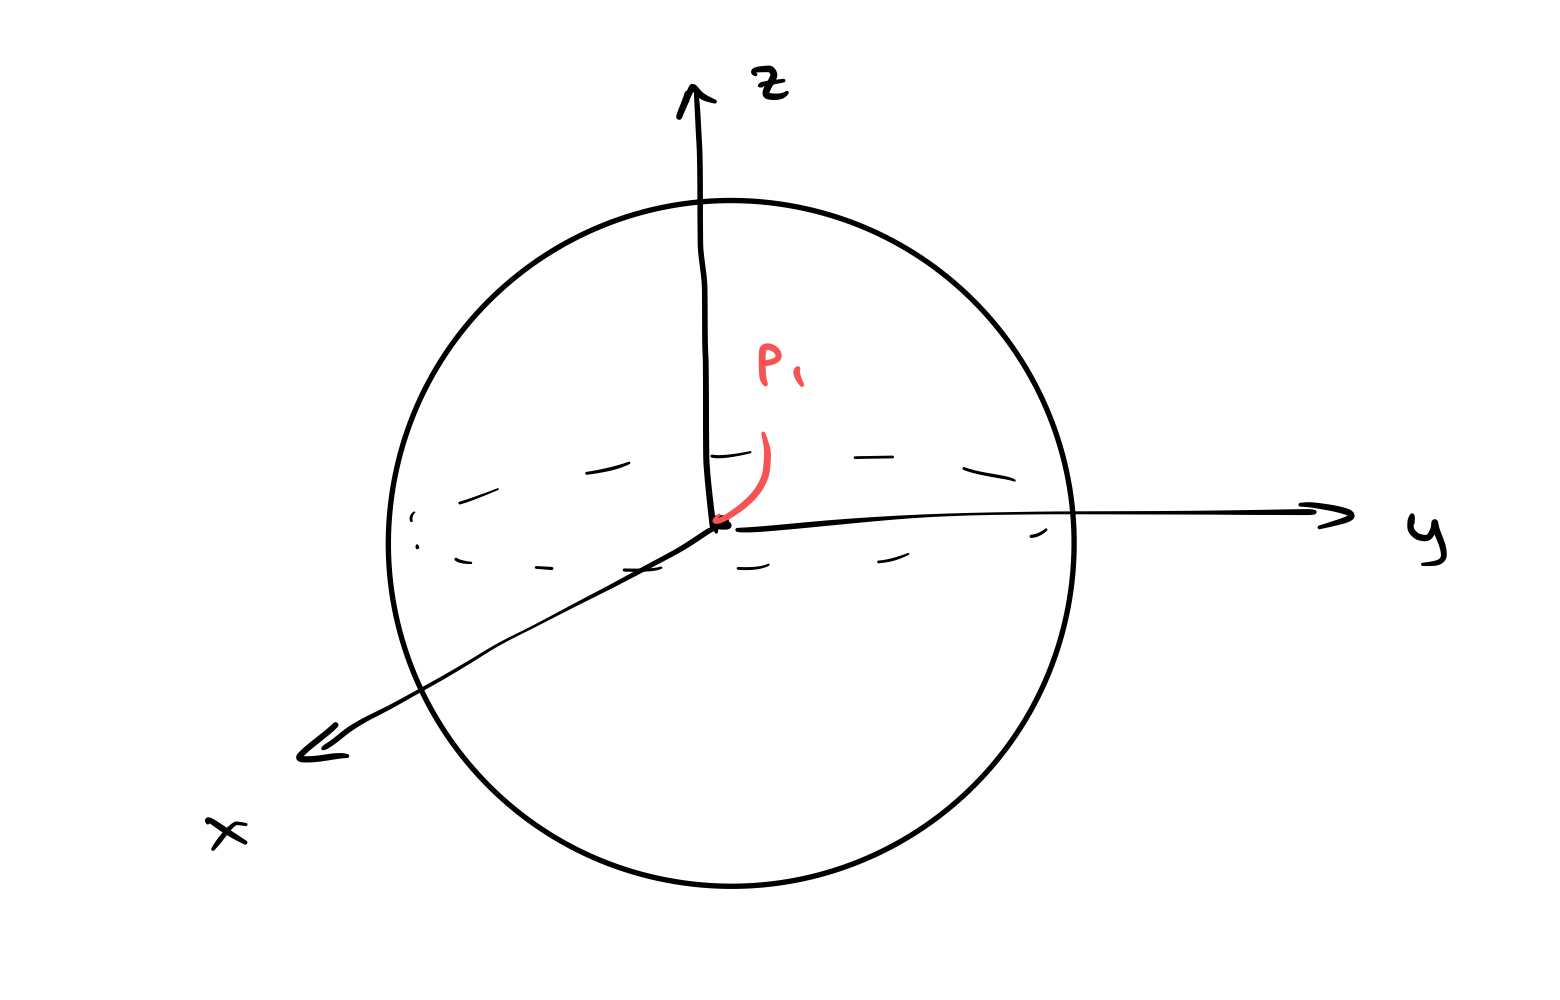
\includegraphics[scale=0.2]{q3a.jpeg}
				\end{center}
			\end{solution}
		\item \( \rho_2 = \frac{3}{4}\ket*{0} \bra*{0} + \frac{1}{4}X\ket*{0} \bra*{0} X^{\dagger}\) 

			\begin{solution}
				Again, following the same steps as earlier:
				\[
					\rho_2 = \begin{pmatrix} \frac{3}{4} & 0 \\ 0 & 0 \end{pmatrix} 
				\] 
				Therefore:
				\begin{align*}
					\mean X_{\rho} &= 0 \\
					\mean Y_{\rho}&= 0 \\
					\mean Z_{\rho} &= \frac{3}{4} 
				\end{align*}
				The diagram:
				\begin{center}
					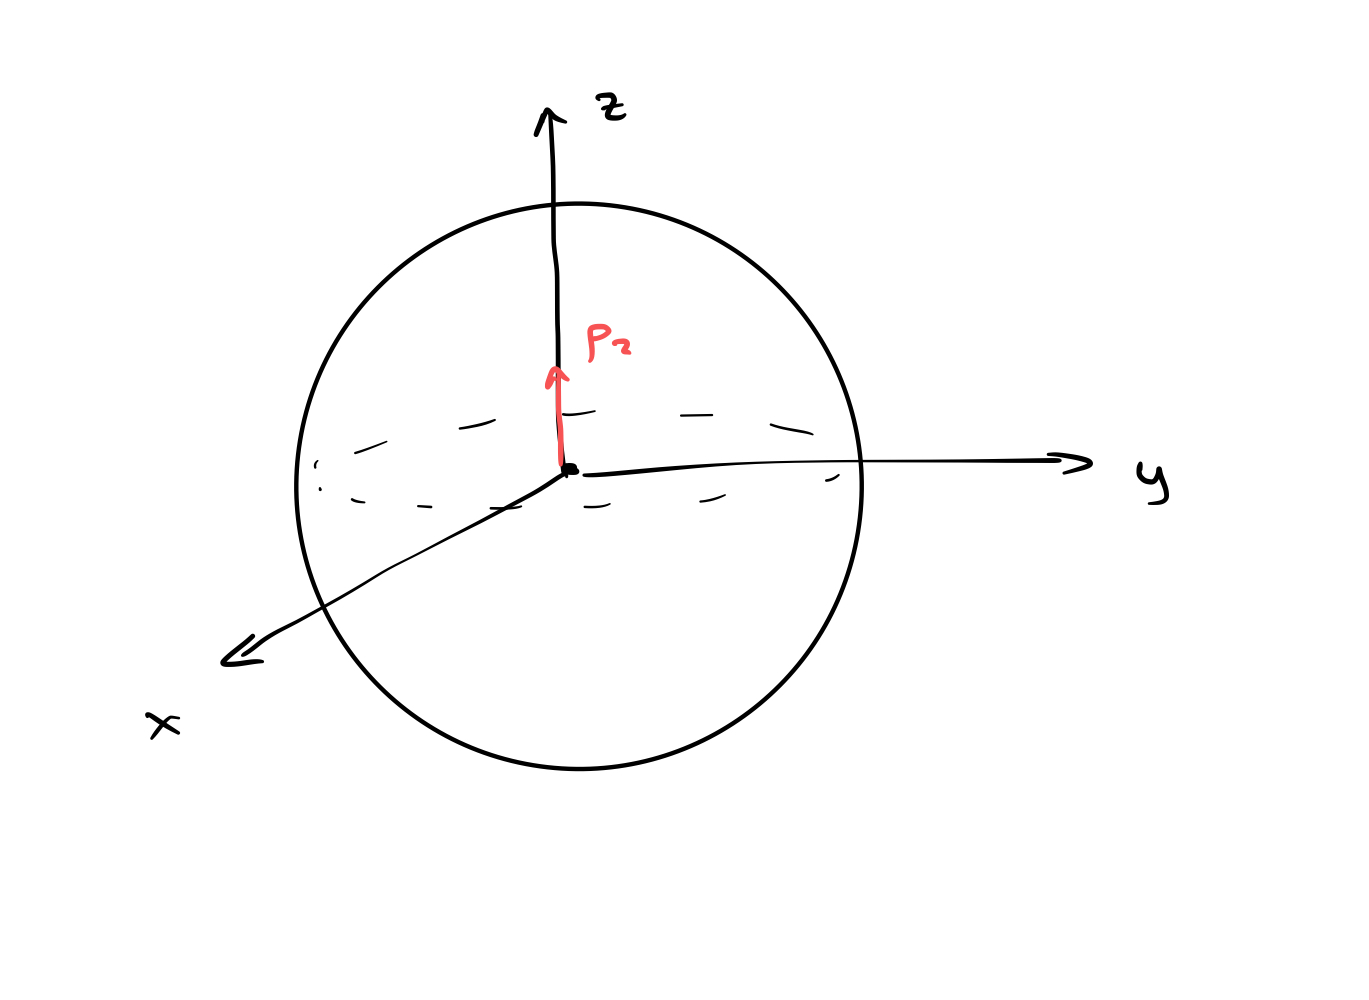
\includegraphics[scale=0.2]{q3b.jpeg}
				\end{center}
			\end{solution}
		\item \( \rho_3 = \frac{3}{4}\ket*{+}\bra*{+} + \frac{1}{4}Z \ket*{+}\bra*{+}Z^{\dagger}\)

			\begin{solution}
				As before, we have:
				\[
					\rho_3 = \begin{pmatrix} 1 / 2 & 3 / 8 \\ 3 / 8 & 1 / 2 \end{pmatrix} 
				\] 
				Therefore:
				\begin{align*}
					\mean X_{\rho} &= \frac{3}{4} \\
					\mean Y_{\rho}&= 0 \\
					\mean Z_{\rho} &= 0 
				\end{align*}
				Diagram:
				\begin{center}
					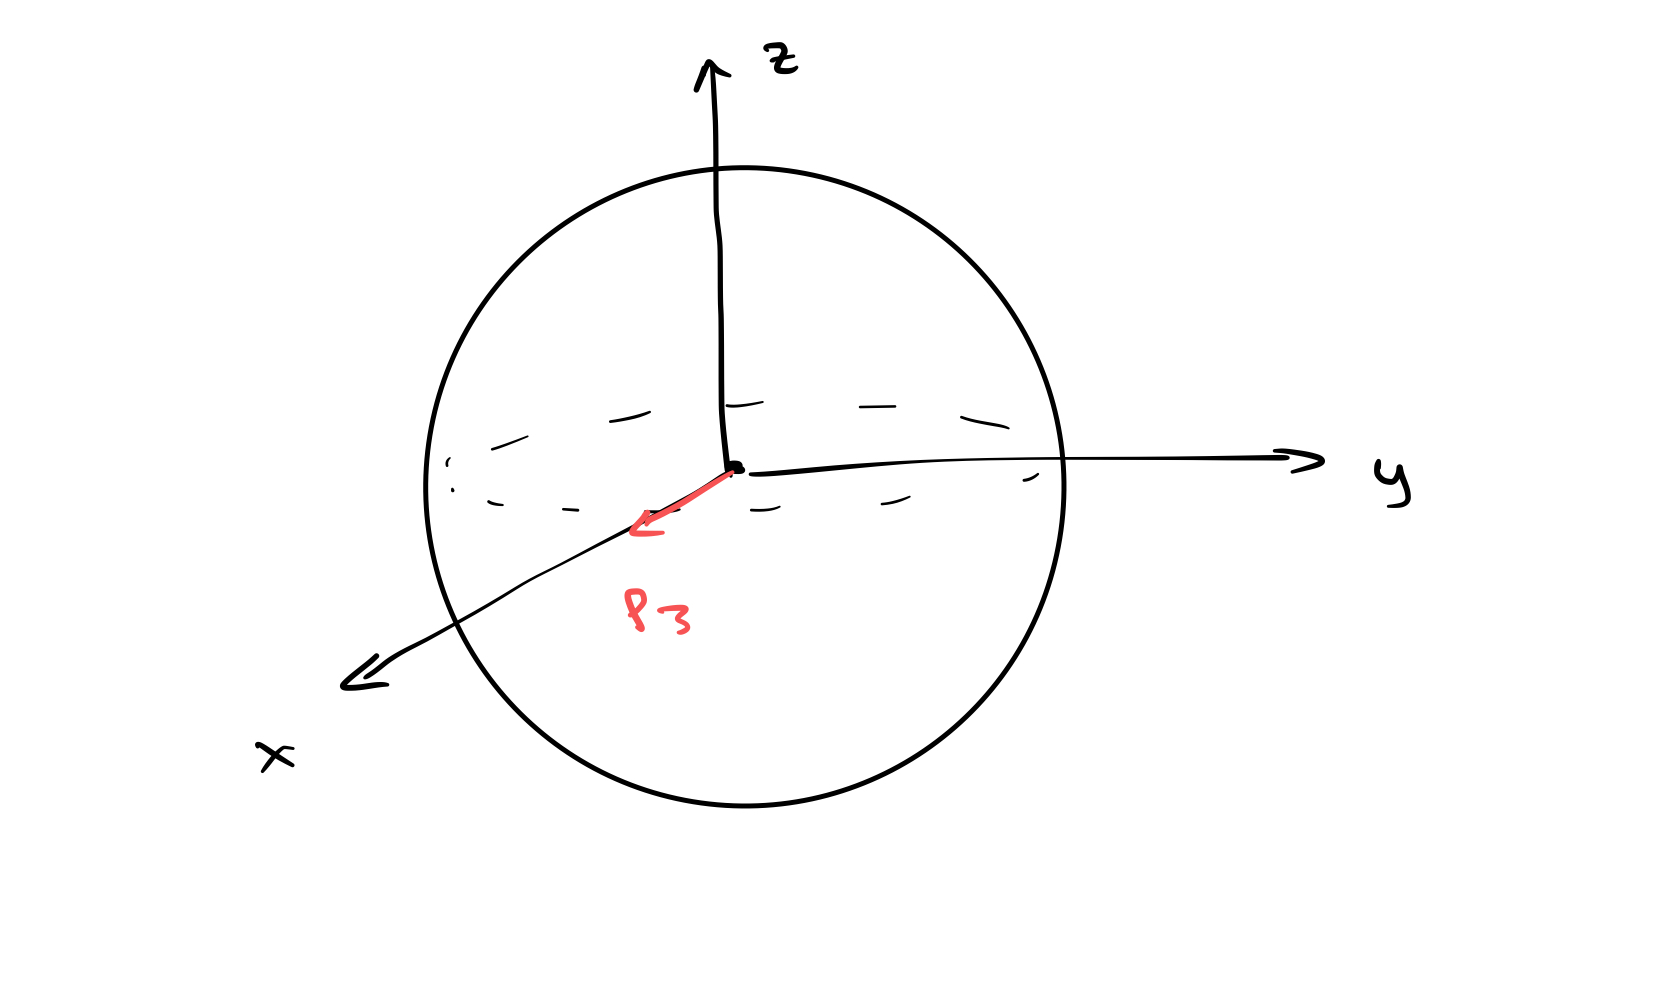
\includegraphics[scale=0.2]{q3c.jpeg}
				\end{center}
			\end{solution}
	 \end{enumerate}
\end{document}
